\documentclass[lualatex,ja=standard,a4paper,12pt]{bxjsarticle}
\usepackage{amsmath, amssymb, amsthm}
\usepackage{geometry}
\usepackage{xcolor}
\usepackage{tcolorbox}
\usepackage{booktabs}
\usepackage{array}
\usepackage{graphicx}
\usepackage{listings}
\usepackage{tikz}
\usetikzlibrary{arrows.meta, positioning}

\geometry{margin=25mm}

\tcbuselibrary{theorems, skins, breakable}

\newtcolorbox{defbox}[1]{
  colback=blue!5, colframe=blue!60!black,
  fonttitle=\bfseries, title={#1}, arc=3pt, breakable
}
\newtcolorbox{thmbox}[1]{
  colback=green!5, colframe=green!50!black,
  fonttitle=\bfseries, title={#1}, arc=3pt, breakable
}
\newtcolorbox{pointbox}{
  colback=orange!8, colframe=orange!70!black,
  fonttitle=\bfseries, title={ポイント}, arc=3pt, breakable
}
\newtcolorbox{exbox}[1]{
  colback=gray!6, colframe=gray!50,
  fonttitle=\bfseries, title={例：#1}, arc=3pt, breakable
}
\newtcolorbox{warningbox}{
  colback=red!5, colframe=red!60!black,
  fonttitle=\bfseries, title={注意}, arc=3pt, breakable
}

\lstset{
  basicstyle=\ttfamily\small,
  frame=single,
  framesep=6pt,
  rulecolor=\color{gray!50},
  backgroundcolor=\color{gray!4},
  breaklines=true,
  showstringspaces=false,
  columns=flexible,
}

\title{{\large Hoff 第6章} \\[6pt]
       \textbf{6.6\; Introduction to MCMC Diagnostics} \\[4pt]
       {\normalsize （MCMC診断入門）＋ 6.7 議論と文献\quad ゼミ資料}}
\author{}
\date{}

\begin{document}
\maketitle
\thispagestyle{empty}

% ===========================
\section{何を診断したいのか}
% ===========================

モンテカルロ近似・MCMC近似の目的は，
関心のある任意の関数 $g$ について
\[
  \frac{1}{S}\sum_{s=1}^{S} g(\phi^{(s)})
  \;\approx\; \int g(\phi)\, p(\phi)\, d\phi
\]
が成り立つような列 $\{\phi^{(1)}, \ldots, \phi^{(S)}\}$ を得ることであった．
これが\textbf{幅広い $g$ について}よい近似であるためには，
生成された列の\textbf{経験分布が目標分布 $p(\phi)$ に似ている}必要がある．

\medskip
列を作る方法は2つあった．両者の保証の強さを比べると：

\begin{center}
\renewcommand{\arraystretch}{1.8}
\begin{tabular}{lll}
\toprule
 & 独立モンテカルロ（MC） & MCMC \\
\midrule
保証されること
  & $\Pr(\phi^{(s)} \in A) = \int_A p(\phi)\,d\phi$
  & $\displaystyle\lim_{s\to\infty}\Pr(\phi^{(s)} \in A) = \int_A p(\phi)\,d\phi$ \\
いつ成り立つか
  & \textbf{すべての $s$} で成立
  & $s \to \infty$ の\textbf{極限でのみ} \\
他の標本との関係
  & 条件付きでも無条件でも成立
  & 直前の標本に依存する \\
\bottomrule
\end{tabular}
\end{center}

\medskip
\noindent 独立MC標本は，列が $p(\phi)$ を代表することが\textbf{自動的に}保証される
——その意味で\textbf{「ゴールドスタンダード」}である．
MCMCではそれが言えない．言えるのは極限のことだけである．

\medskip
では有限の $S$ で止めるとき，何が起こりうるのか．
極端な例を1つ見る．

% ===========================
\section{例：正規混合分布でMCとMCMCを比べる}
% ===========================

\begin{exbox}{3成分の正規混合}
2つの変数の同時分布を目標分布とする：
離散変数 $\delta \in \{1,2,3\}$ と連続変数 $\theta \in \mathbb{R}$．
\begin{align*}
  \{\Pr(\delta=1), \Pr(\delta=2), \Pr(\delta=3)\} &= (0.45,\ 0.10,\ 0.45), \\[4pt]
  p(\theta \mid \delta) &= \mathrm{dnorm}(\theta,\ \mu_\delta,\ \sigma_\delta)
\end{align*}
ただし $(\mu_1, \mu_2, \mu_3) = (-3, 0, 3)$，
$(\sigma_1^2, \sigma_2^2, \sigma_3^2) = (1/3,\ 1/3,\ 1/3)$．

\medskip
$\delta$ を\textbf{グループ所属を表す変数}，
$(\mu_\delta, \sigma_\delta^2)$ をグループ $\delta$ の母平均・母分散と考えればよい．
$\theta$ の周辺密度 $p(\theta) = \sum_\delta p(\theta \mid \delta)p(\delta)$ は
3つのグループ平均に対応する\textbf{3つの峰}を持つ．
\end{exbox}

\subsection*{独立モンテカルロなら簡単}

$\phi = (\delta, \theta)$ の同時分布からの独立標本は簡単に得られる：
\begin{enumerate}
  \item $\delta$ をその周辺分布 $(0.45, 0.10, 0.45)$ から引く
  \item その $\delta$ を $p(\theta \mid \delta)$ に代入して $\theta$ を引く
\end{enumerate}
得られたペア $(\delta, \theta)$ は
$p(\delta, \theta) = p(\delta)p(\theta \mid \delta)$ からの標本である
（6.3節の\textbf{合成の原理}そのもの）．

\begin{figure}[htbp]
\centering
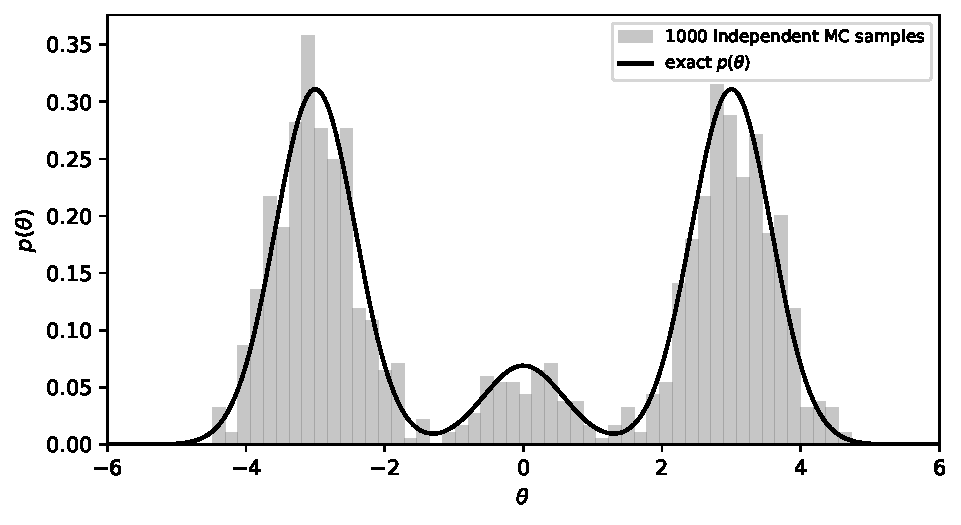
\includegraphics[width=0.75\textwidth]{fig6_4.pdf}
\caption{正規混合の真の密度（黒線）と，1000個の独立モンテカルロ標本のヒストグラム．
Hoff の Figure 6.4 に対応．}
\end{figure}

\noindent 経験分布は $p(\theta)$ に\textbf{よく似ている}．3つの峰の高さの比も正しい．

\subsection*{ギブスサンプラーを組む}

同じ分布に対してギブスサンプラーも簡単に作れる．
$\theta$ の完全条件付き分布はすでに与えられている
（$p(\theta \mid \delta) = \mathrm{dnorm}(\theta, \mu_\delta, \sigma_\delta)$）．
$\delta$ のほうはベイズの定理から
\[
  \Pr(\delta = d \mid \theta)
  = \frac{\Pr(\delta = d) \times \mathrm{dnorm}(\theta,\ \mu_d,\ \sigma_d)}
         {\sum_{d=1}^{3} \Pr(\delta = d) \times \mathrm{dnorm}(\theta,\ \mu_d,\ \sigma_d)},
  \qquad d \in \{1,2,3\}.
\]
あとは $\theta$ と $\delta$ を交互に引くだけである．

\begin{figure}[htbp]
\centering
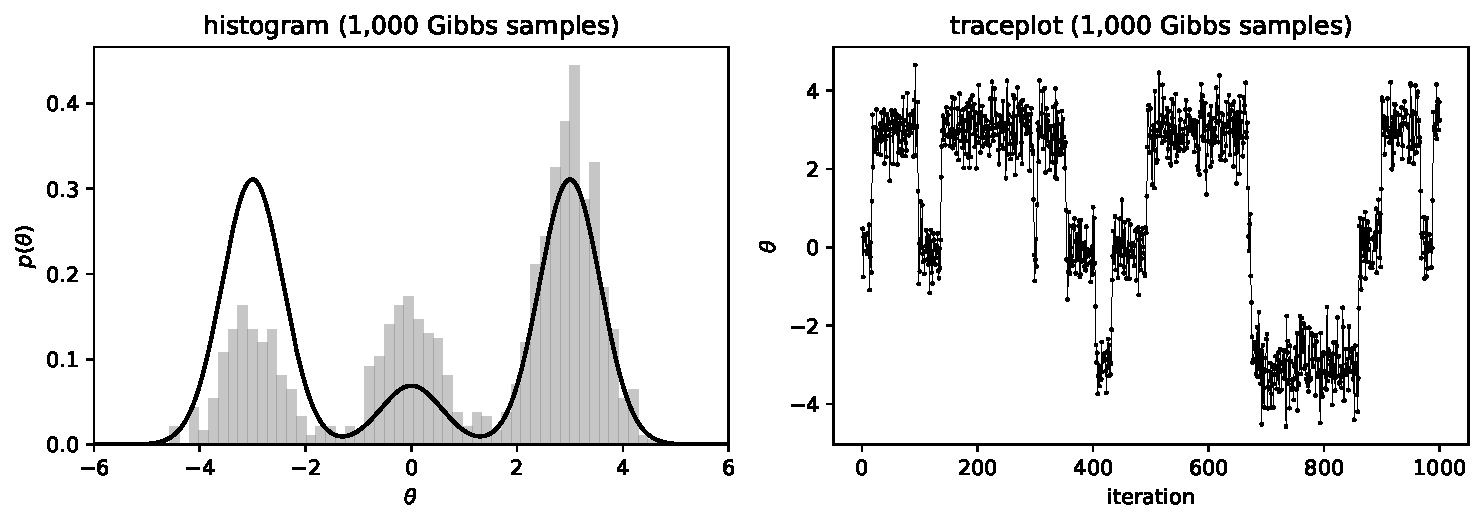
\includegraphics[width=\textwidth]{fig6_5.pdf}
\caption{1000個のギブス標本のヒストグラム（左）とトレースプロット（右）．
Hoff の Figure 6.5 に対応．}
\end{figure}

\begin{warningbox}
\textbf{うまくいっていない}

左のヒストグラムは $p(\theta)$ の\textbf{ひどい近似}である：
\begin{itemize}
  \item $\theta \approx -3$ の値が\textbf{過小}に現れている
  \item $\theta \approx 0$ と $\theta \approx +3$ の値が\textbf{過大}に現れている
\end{itemize}
独立MCではまったく同じ分布がきれいに再現できていたのに，である．
\end{warningbox}

\subsection*{トレースプロットが語ること}

何が起きたかは右のトレースプロット（反復番号に対して $\theta$ の値を描いたもの）を
見れば分かる．
$\theta$ の値は\textbf{ある領域に「はまり込み」}，
3つの $\mu$ が表す領域の間を\textbf{めったに移動しない}．

\begin{defbox}{自己相関（autocorrelation）}
この「ねばつき」（stickiness）を表す専門用語が\textbf{自己相関}，
すなわち連鎖の\textbf{連続する値どうしの相関}である．
\end{defbox}

\begin{pointbox}
\textbf{なぜねばつくのか——悪循環の構造}

このギブスサンプラーでは：
\begin{itemize}
  \item $\theta$ が 0 の近くにあれば，次の $\delta$ はほぼ確実に 2 になる
  \item $\delta$ が 2 なら，次の $\theta$ はほぼ確実に 0 の近くになる
\end{itemize}
その結果，連続する $\theta$ の値のあいだに\textbf{強い正の相関}が生じる．

\medskip
数値で見ると，$\theta = 0$ のとき
$\mathrm{dnorm}(0, \pm 3, 1/\sqrt{3})$ は
$\mathrm{dnorm}(0, 0, 1/\sqrt{3})$ の $10^{-6}$ 倍程度しかない．
$\delta$ が 1 や 3 に移るには，まず $\theta$ が
$\mathrm{Normal}(0, 1/3)$ の\textbf{遠い裾}（$\theta \approx 1.5$ 付近）
まで飛ぶ必要がある．それは数百反復に1回しか起きない．

\medskip
峰どうしが離れているほど，また峰が鋭いほど，この問題は深刻になる．
\end{pointbox}

\subsection*{「いつかは収束する」の「いつか」}

ギブスサンプラーは\textbf{いずれ}よい近似を与えると保証されていたはずではないか
（6.5節の主張1）．
その通りである．しかし状況によっては\textbf{「いずれ」が非常に長い}．

\begin{figure}[htbp]
\centering
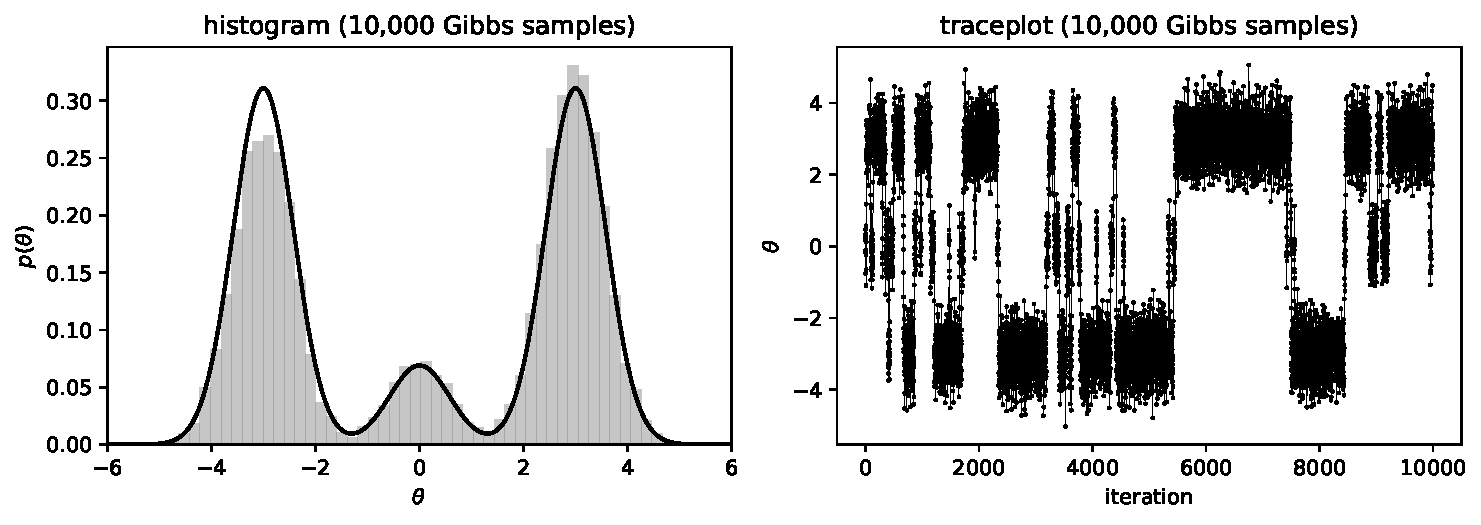
\includegraphics[width=\textwidth]{fig6_6.pdf}
\caption{10,000個のギブス標本．1000個のときより大幅に改善したが，
まだやや不十分である．Hoff の Figure 6.6 に対応．}
\end{figure}

\noindent 10倍回しても「かなり良くなったが，まだ少し足りない」程度である．

% ===========================
\section{粒子のたとえ：定常性と混合}
% ===========================

一般のパラメータ $\phi$ と目標分布 $p(\phi)$ について，
列 $\{\phi^{(1)}, \ldots, \phi^{(S)}\}$ を
\textbf{パラメータ空間を動き回る粒子 $\phi$ の軌跡}と考えると見通しがよい．

\begin{thmbox}{MCMC近似にとって決定的なこと}
粒子が\textbf{ある集合 $A$ に滞在する時間}が，
目標確率 $\int_A p(\phi)\,d\phi$ に\textbf{比例している}こと．
\end{thmbox}

\medskip
いま $A_1, A_2, A_3$ を互いに交わらない3つの部分集合とし，
$\Pr(A_2) < \Pr(A_1) \approx \Pr(A_3)$ とする
（上の正規混合の3つの峰のまわりだと思えばよい）．
積分近似の観点からは，粒子には
\textbf{$A_2$ での滞在は短く，$A_1$ と $A_3$ では同じくらい}
滞在してほしい．

\medskip
ところが一般に $p(\phi)$ は分かっていない（分かっていれば近似する必要がない）．
したがって\textbf{たまたま $A_2$ から連鎖を始めてしまう}ことがありうる．
その場合，反復数 $S$ は粒子が次の2つを行う余裕があるくらい大きくなければならない：

\begin{enumerate}
  \item $A_2$ から抜け出し，より確率の高い領域へ移る
  \item $A_1$ と $A_3$ の間，およびその他の高確率領域の間を行き来する
\end{enumerate}

\begin{defbox}{定常性（stationarity）と混合（mixing）}
\begin{itemize}
  \item 項目1が達成されることを，連鎖が\textbf{定常性に達した}
        あるいは\textbf{収束した}（converged）という．
  \item 項目2に関わる「粒子がどれだけ速くパラメータ空間を動き回るか」を
        \textbf{混合の速さ}（speed of mixing）と呼ぶ．
\end{itemize}

\medskip
独立MCサンプラーは\textbf{完璧な混合}を持つ：
自己相関はゼロで，1ステップでパラメータ空間の別の領域へ飛べる．
\end{defbox}

\begin{warningbox}
\textbf{収束したことは確かめられない}

高確率の領域から始められたなら，収束は普通あまり問題にならない．
しかし\textbf{よい領域から始めたかどうか分からない}場合，
収束の判定は\textbf{認識論的な困難}をはらむ．

\medskip
Hoff の言い方が正確である：
\begin{quote}
一般に，連鎖が収束した\textbf{かどうかを確実に知ることはできない}．
しかし収束して\textbf{いない}ことなら分かる場合がある．
だからせめて後者を確認する．
\end{quote}

\medskip
確認することの1つが\textbf{定常性}，すなわち
連鎖のある部分から取った標本が，
別の部分から取った標本と似た分布を持つかどうかである．
\end{warningbox}

\medskip
\noindent 6.4節の半共役正規モデルでは，定常性はごく速やかに達成され問題にならない．
しかし後の章で出てくる\textbf{パラメータの多いモデル}では，
自己相関が高く，よい出発点を見つけるのが難しく，
定常性に達するまで長くかかることがある．
そうした場合はMCMCサンプラーを\textbf{非常に長く}走らせる必要がある．

% ===========================
\section{自己相関は近似精度をどう悪化させるか}
% ===========================

ここを定量化する．
$E[\phi] = \int \phi\, p(\phi)\, d\phi = \phi_0$ を
$\{\phi^{(1)}, \ldots, \phi^{(S)}\}$ の経験分布で近似したいとする．

\subsection*{独立MCの場合}

$\phi$ の値が $p(\phi)$ からの独立標本なら，
$\bar{\phi} = \sum \phi^{(s)}/S$ の分散は
\[
  \mathrm{Var}_{\mathrm{MC}}[\bar{\phi}]
  = E[(\bar{\phi} - \phi_0)^2]
  = \frac{\mathrm{Var}[\phi]}{S},
  \qquad
  \mathrm{Var}[\phi] = \int \phi^2 p(\phi)\, d\phi - \phi_0^2.
\]
その平方根が第4章の\textbf{モンテカルロ標準誤差}であり，
$\bar{\phi}$ が積分をどれだけうまく近似するかの尺度になる．
MC近似を何度もやり直せば，真値 $\phi_0$ は区間
$\bar{\phi} \pm 2\sqrt{\mathrm{Var}_{\mathrm{MC}}[\bar{\phi}]}$ に
おおよそ95\%の割合で含まれる．
この区間の幅 $4\sqrt{\mathrm{Var}_{\mathrm{MC}}[\bar{\phi}]}$ は
\textbf{標本を増やせばいくらでも小さくできる}．

\subsection*{MCMCの場合}

図6.5・6.6で見たように，連続するMCMC標本 $\phi^{(s)}$ と $\phi^{(s+1)}$ は
正に相関しうる．定常性が達成されているとして，
近似 $\bar{\phi}$ と目標 $\phi_0$ の期待二乗差を計算すると：

\begin{align*}
  \mathrm{Var}_{\mathrm{MCMC}}[\bar{\phi}]
  &= E[(\bar{\phi} - \phi_0)^2] \\
  &= E\!\left[\Big\{\tfrac{1}{S}\textstyle\sum (\phi^{(s)} - \phi_0)\Big\}^2\right] \\
  &= \frac{1}{S^2} E\!\left[\sum_{s=1}^{S}(\phi^{(s)} - \phi_0)^2
      + \sum_{s \ne t}(\phi^{(s)} - \phi_0)(\phi^{(t)} - \phi_0)\right] \\
  &= \frac{1}{S^2}\sum_{s=1}^{S} E[(\phi^{(s)} - \phi_0)^2]
      + \frac{1}{S^2}\sum_{s \ne t} E[(\phi^{(s)} - \phi_0)(\phi^{(t)} - \phi_0)] \\
  &= \mathrm{Var}_{\mathrm{MC}}[\bar{\phi}]
      + \frac{1}{S^2}\sum_{s \ne t} E[(\phi^{(s)} - \phi_0)(\phi^{(t)} - \phi_0)].
\end{align*}

\begin{thmbox}{結論}
\[
  \mathrm{Var}_{\mathrm{MCMC}}[\bar{\phi}]
  = \underbrace{\mathrm{Var}_{\mathrm{MC}}[\bar{\phi}]}_{\text{独立なら これだけ}}
  + \underbrace{\frac{1}{S^2}\sum_{s \ne t} E[(\phi^{(s)} - \phi_0)(\phi^{(t)} - \phi_0)]}_{\text{連鎖内の相関による項}}
\]
この追加項は\textbf{一般に正}なので，MCMC分散はMC分散より大きい．
つまりMCMC近似はMC近似よりも $\phi_0$ から\textbf{遠い}と予想される．
\textbf{自己相関が高いほどMCMC分散は大きく，近似は悪くなる．}
\end{thmbox}

\begin{pointbox}
\textbf{独立なら消える項}

独立標本なら $s \ne t$ について
$E[(\phi^{(s)} - \phi_0)(\phi^{(t)} - \phi_0)] = 0$ なので，
追加項はきれいに消えて $\mathrm{Var}[\phi]/S$ だけが残る．
つまり上の式は\textbf{MCの公式を特別な場合として含んでいる}．

\medskip
また，追加項が正になるのは\textbf{正の自己相関}があるときである．
原理的には負の自己相関を持つ連鎖なら
独立標本より\textbf{良く}なりうるが，
ギブスサンプラーで通常現れるのは正の相関のほうである．
\end{pointbox}

% ===========================
\section{診断の道具}
% ===========================

\subsection*{標本自己相関関数}

連鎖にどれだけ相関があるかを測るには\textbf{標本自己相関関数}を計算する．
一般の数列 $\{\phi_1, \ldots, \phi_S\}$ について，
\textbf{ラグ $t$ の自己相関関数}は $t$ ステップ離れた要素どうしの相関を推定する：

\begin{defbox}{ラグ $t$ の標本自己相関}
\[
  \mathrm{acf}_t(\boldsymbol{\phi})
  = \frac{\frac{1}{S-t}\sum_{s=1}^{S-t}(\phi_s - \bar{\phi})(\phi_{s+t} - \bar{\phi})}
         {\frac{1}{S-1}\sum_{s=1}^{S}(\phi_s - \bar{\phi})^2}
\]
R では関数 \texttt{acf} で計算できる．
\end{defbox}

\noindent 図6.6の10,000個の $\theta$ の列では，
\textbf{ラグ10の自己相関が 0.93，ラグ50の自己相関が 0.812} である．

\begin{warningbox}
これほど自己相関の高いマルコフ連鎖は，パラメータ空間を\textbf{ゆっくりとしか動かない}．
したがって各領域の正しいバランスに達するまで長い時間がかかる．
自己相関が高いほど，与えられた精度を得るのに必要な標本数は増える．
\end{warningbox}

\subsection*{有効標本サイズ}

必要な標本数の増加を測る方法の1つが\textbf{有効標本サイズ}である．

\begin{defbox}{有効標本サイズ（effective sample size）}
\[
  \mathrm{Var}_{\mathrm{MCMC}}[\bar{\phi}] = \frac{\mathrm{Var}[\phi]}{S_{\mathrm{eff}}}
\]
を満たす $S_{\mathrm{eff}}$ を有効標本サイズと呼ぶ．
これは
\textbf{「MCMC標本と同じ精度を与えるのに必要な独立モンテカルロ標本の個数」}
と解釈できる．
R では \texttt{coda} パッケージの \texttt{effectiveSize} で計算する．
\end{defbox}

\begin{warningbox}
\textbf{正規混合の例の衝撃的な数字}

10,000個のギブス標本の有効標本サイズは \textbf{18.42} である．

\medskip
すなわち，$E[\theta]$ のMCMC近似の精度は，
$\theta$ の\textbf{独立標本わずか18個ぶん}でしかない．
1万回まわして18個である．
\end{warningbox}

% ===========================
\section{半共役正規モデルの診断}
% ===========================

では6.4節のギブスサンプラー（$\theta$ と $\sigma^2$）はどうだったのか．

\begin{figure}[htbp]
\centering
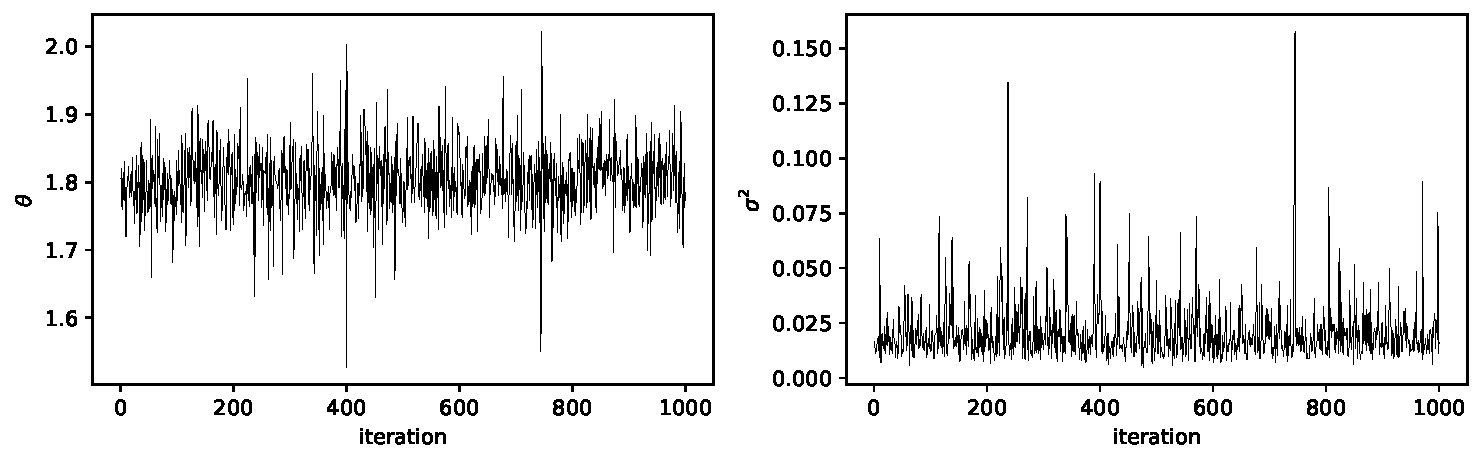
\includegraphics[width=\textwidth]{fig6_7.pdf}
\caption{6.4節のギブスサンプラーの $\theta$ と $\sigma^2$ のトレースプロット．
Hoff の Figure 6.7 に対応．}
\end{figure}

\noindent 値を順番に並べたこの図は，
\textbf{ただちに収束していること}と\textbf{自己相関が低いこと}を示している．
図6.5の「はまり込む」トレースプロットと見比べたい．

\begin{center}
\renewcommand{\arraystretch}{1.5}
\begin{tabular}{llrr}
\toprule
 & & ラグ1の自己相関 & 有効標本サイズ \\
\midrule
$\theta$   & Hoff（R，\texttt{coda}） & 0.031 & 1000 \\
           & 再現（Python）           & $-0.024$ & 1000 \\
\midrule
$\sigma^2$ & Hoff（R，\texttt{coda}） & 0.147 & 742 \\
           & 再現（Python）           & 0.240 & 598 \\
\bottomrule
\end{tabular}
\end{center}

\medskip
\noindent $\theta$ のラグ1自己相関 0.031 は，近似の目的には\textbf{実質ゼロ}である．
有効標本サイズは 1,000，つまり\textbf{1000個の標本が1000個ぶん働いている}．
$\sigma^2$ は自己相関 0.147，有効標本サイズ 742 とやや劣るが十分よい．

\medskip
独立に引いた列ほどではないにせよ，
\textbf{このモデルと事前分布に対するギブスサンプラーは非常にうまく機能している}．

\begin{pointbox}
\textbf{再現値のズレについて}

$\sigma^2$ の値が Hoff（0.147 / 742）と再現（0.240 / 598）でずれているのは，
乱数生成器が違うことに加え，
$S = 1000$ での自己相関や有効標本サイズの推定自体が
\textbf{かなりばらつく}ためである．
有効標本サイズの計算法も，\texttt{coda} はARスペクトル法，
再現コードは Geyer の初期正値列による打ち切りで，実装が異なる．

\medskip
一方，正規混合の例（10,000標本）では
ラグ10が 0.929 対 0.93，ラグ50が 0.809 対 0.812，
有効標本サイズが 19.4 対 18.42 とよく一致する．
\textbf{標本数が多いほど診断量の推定も安定する}という当たり前のことが効いている．
\end{pointbox}

\begin{pointbox}
\textbf{この2つの例の対比が6.6節の主題である}

\begin{center}
\renewcommand{\arraystretch}{1.5}
\begin{tabular}{lll}
\toprule
 & 正規混合 & 半共役正規モデル \\
\midrule
反復数 & 10,000 & 1,000 \\
ラグ1の自己相関 & 非常に高い & $\approx 0$ \\
有効標本サイズ & 18 & 1000 \\
評価 & \textbf{ほぼ役に立たない} & \textbf{独立標本とほぼ同等} \\
\bottomrule
\end{tabular}
\end{center}

\medskip
\textbf{同じギブスサンプラーという手法でも，対象によって性能は桁違いに変わる．}
6.5節の収束定理は両方に等しく当てはまるが，
それは有限回で使えるかどうかを何も語らない．
だから毎回\textbf{診断しなければならない}．
\end{pointbox}

% ===========================
\section{6.7\; 議論と文献}
% ===========================

\paragraph{用語と歴史}
「ギブスサンプリング」という語は
\textbf{Geman and Geman (1984)} の画像解析の論文で作られた．
ただしアルゴリズム自体はそれ以前に空間統計の文脈で現れており，
たとえば \textbf{Besag (1974)} や \textbf{Ripley (1979)} がある．
しかしベイズのデータ解析におけるギブスサンプラーの一般的な有用性が
十分に認識されたのは1980年代末
（\textbf{Gelfand and Smith, 1990}）になってからである．
歴史的な総説としては \textbf{Robert and Casella (2008)} を参照．

\paragraph{収束診断}
ギブスサンプラーの収束とMCMC近似の精度を評価するのは難しい．
いくつかの収束診断が提案されている
（\textbf{Gelman and Rubin, 1992}；\textbf{Geweke, 1992}；
\textbf{Raftery and Lewis, 1992}）が，
これらは\textbf{問題を指摘できるだけで，よい近似であることを保証はしない}
（\textbf{Geyer, 1992}）．

\paragraph{実践的な入門}
MCMCの実装と評価については大きな文献がある．
手を動かした経験と読書を併せるのがよい．
最初に読む論文として
\textbf{``Practical Markov chain Monte Carlo'' (Geyer, 1992)} が挙げられている．
多くの研究者による討論を含み，MCMC近似に対する多様な視点と技法が示されている．

\begin{warningbox}
\textbf{診断の限界}

6.7節の記述が，6.6節の認識論的な注意と呼応していることに注意したい．
\begin{itemize}
  \item 収束したことは確かめられない（6.6節）
  \item 診断は問題を指摘できるだけで，良さを保証しない（6.7節，Geyer 1992）
\end{itemize}
つまりMCMC診断は\textbf{反証の道具であって，証明の道具ではない}．
「診断を通った」は「大丈夫」を意味しない．
\end{warningbox}

% ===========================
\section{まとめ}
% ===========================

\begin{thmbox}{6.6--6.7節のまとめ}
\begin{enumerate}
  \item 独立MC標本は\textbf{すべての $s$} で目標分布を代表するが，
        MCMC標本について言えるのは\textbf{$s \to \infty$ の極限}だけである．

  \item 正規混合の例では，独立MCは1000標本できれいに近似できるのに，
        ギブスサンプラーは10,000標本でもまだ不十分だった．
        原因は\textbf{自己相関}（連鎖が領域に「はまり込む」こと）．

  \item 粒子のたとえでは，必要なのは
        \textbf{(1) 低確率領域から抜け出すこと（定常性・収束）}と
        \textbf{(2) 高確率領域の間を行き来すること（混合）}である．
        収束したことは確かめられないが，収束していないことは分かる場合がある．

  \item 精度の悪化は
        $\mathrm{Var}_{\mathrm{MCMC}}[\bar{\phi}]
        = \mathrm{Var}_{\mathrm{MC}}[\bar{\phi}] + (\text{相関項})$
        として定量化される．
        道具は\textbf{自己相関関数}（\texttt{acf}）と
        \textbf{有効標本サイズ}（\texttt{effectiveSize}）．

  \item 正規混合では10,000標本の有効標本サイズが\textbf{18}，
        半共役正規モデルでは1,000標本の有効標本サイズが\textbf{1000}（$\theta$）と
        \textbf{742}（$\sigma^2$）であった．
        \textbf{同じ手法でも対象次第で性能は桁違いに変わる}ので，毎回診断する．
\end{enumerate}
\end{thmbox}

\paragraph{第6章全体の流れ}
\begin{center}
\renewcommand{\arraystretch}{1.4}
\begin{tabular}{ll}
\toprule
6.1 & 半共役事前分布 $\to$ $\sigma^2$ の周辺事後が非標準になり，直接引けない \\
6.2 & 離散近似で解決を試みる $\to$ グリッドの配置と次元の呪いで破綻 \\
6.3 & 完全条件付き分布を交互に使う着想 $\to$ 出発点が循環 \\
6.4 & \textbf{ギブスサンプラー}：出発点は適当でよいと割り切る $\to$ 実例で成功 \\
6.5 & 一般形・マルコフ連鎖・収束定理 $\to$ 循環が正式に解消 \\
6.6 & 有限の $S$ での信頼性 $\to$ 自己相関・有効標本サイズによる診断 \\
\bottomrule
\end{tabular}
\end{center}

\end{document}
